% Minimal sebenta template generated automatically
\documentclass[11pt,a4paper]{article}
\usepackage[utf8]{inputenc}
\usepackage[T1]{fontenc}
\usepackage{lmodern}
\usepackage{geometry}
\usepackage{fancyhdr}
\usepackage{hyperref}
\usepackage{graphicx}
\usepackage{float}
\usepackage{placeins}
\usepackage{bookmark}
\usepackage{booktabs}
\usepackage{amsmath,amssymb}
\usepackage{csquotes}
\usepackage{enumitem}
\usepackage{tikz}
\IfFileExists{pgfplots.sty}{\usepackage{pgfplots}\pgfplotsset{compat=1.17}}{}

\geometry{margin=2.5cm}

% Try to include project-specific style macros (containing \exercicio, \subexercicio, etc.)
% Try multiple relative locations to be robust across different generated output paths
\IfFileExists{../../../../Teste_modelo/config/style.tex}{% Sistema de exercícios com contadores automáticos
\newcounter{exerciciocount}          % Contador principal dos exercícios
\newcounter{subexerciciocount}       % Contador dos subexercícios
\newcounter{optioncount}             % Contador das opções

% Control whether the macro prints the automatic "Exercício N." heading.
% Default: show the heading. Call \showexerciciotitlefalse to suppress.
\newif\ifshowexerciciotitle
\showexerciciotitletrue

% Macro para exercício principal
\newcommand{\exercicio}[1]{%
        \par\vspace{1.5em}% Espaçamento antes
        \refstepcounter{exerciciocount}% Incrementa contador principal
        \setcounter{subexerciciocount}{0}% Reseta contador de subexercícios
        \setcounter{optioncount}{0}% Reseta contador de opções
        % Only print the automatic heading if the flag is true
        \ifshowexerciciotitle
            \noindent\textbf{Exercício~\theexerciciocount.}\space #1\par\vspace{0.5em}%
        \else
            % When suppressed, just print the content without the heading
            #1\par\vspace{0.5em}%
        \fi
}

% Macro para subexercício
\newcommand{\subexercicio}[1]{%
    \par\vspace{0.8em}% Espaçamento menor para subexercícios
    \refstepcounter{subexerciciocount}% Incrementa contador de subexercícios
    \noindent\textbf{\theexerciciocount.\thesubexerciciocount.} #1\par\vspace{0.3em}%
}

% Macro para opção
\newcommand{\option}[1]{%
    \par
    \refstepcounter{optioncount}%
    \noindent(\alph{optioncount}) #1%
}

% Título e informações do exame
\title{1ª Questão de aula do Módulo A10: Otimização}
\author{EPRALIMA - Escola Profissional Alto Lima}

\date{}

% Cabeçalho completo do teste dentro de uma caixa simples
\newcommand{\espacoAluno}{%
    \vspace{0.5cm}
    \fbox{%
        \parbox{\textwidth}{%
            \noindent\textbf{Nome do Aluno:} \underline{\hspace{7cm}} \textbf{Turma:} \underline{\hspace{1cm}}\\[0.5cm]
            \noindent\textbf{Assinatura do Professor:} \underline{\hspace{3cm}} \hfill \textbf{Nota:} \underline{\hspace{2cm}}\\[0.5cm]
            \noindent\textbf{Assinatura do Encarregado de Educação:} \underline{\hspace{3cm}}
        }%
    }
    \vspace{1cm}
}}{%
  \IfFileExists{../../../Teste_modelo/config/style.tex}{% Sistema de exercícios com contadores automáticos
\newcounter{exerciciocount}          % Contador principal dos exercícios
\newcounter{subexerciciocount}       % Contador dos subexercícios
\newcounter{optioncount}             % Contador das opções

% Control whether the macro prints the automatic "Exercício N." heading.
% Default: show the heading. Call \showexerciciotitlefalse to suppress.
\newif\ifshowexerciciotitle
\showexerciciotitletrue

% Macro para exercício principal
\newcommand{\exercicio}[1]{%
        \par\vspace{1.5em}% Espaçamento antes
        \refstepcounter{exerciciocount}% Incrementa contador principal
        \setcounter{subexerciciocount}{0}% Reseta contador de subexercícios
        \setcounter{optioncount}{0}% Reseta contador de opções
        % Only print the automatic heading if the flag is true
        \ifshowexerciciotitle
            \noindent\textbf{Exercício~\theexerciciocount.}\space #1\par\vspace{0.5em}%
        \else
            % When suppressed, just print the content without the heading
            #1\par\vspace{0.5em}%
        \fi
}

% Macro para subexercício
\newcommand{\subexercicio}[1]{%
    \par\vspace{0.8em}% Espaçamento menor para subexercícios
    \refstepcounter{subexerciciocount}% Incrementa contador de subexercícios
    \noindent\textbf{\theexerciciocount.\thesubexerciciocount.} #1\par\vspace{0.3em}%
}

% Macro para opção
\newcommand{\option}[1]{%
    \par
    \refstepcounter{optioncount}%
    \noindent(\alph{optioncount}) #1%
}

% Título e informações do exame
\title{1ª Questão de aula do Módulo A10: Otimização}
\author{EPRALIMA - Escola Profissional Alto Lima}

\date{}

% Cabeçalho completo do teste dentro de uma caixa simples
\newcommand{\espacoAluno}{%
    \vspace{0.5cm}
    \fbox{%
        \parbox{\textwidth}{%
            \noindent\textbf{Nome do Aluno:} \underline{\hspace{7cm}} \textbf{Turma:} \underline{\hspace{1cm}}\\[0.5cm]
            \noindent\textbf{Assinatura do Professor:} \underline{\hspace{3cm}} \hfill \textbf{Nota:} \underline{\hspace{2cm}}\\[0.5cm]
            \noindent\textbf{Assinatura do Encarregado de Educação:} \underline{\hspace{3cm}}
        }%
    }
    \vspace{1cm}
}}{%
    \IfFileExists{../../Teste_modelo/config/style.tex}{% Sistema de exercícios com contadores automáticos
\newcounter{exerciciocount}          % Contador principal dos exercícios
\newcounter{subexerciciocount}       % Contador dos subexercícios
\newcounter{optioncount}             % Contador das opções

% Control whether the macro prints the automatic "Exercício N." heading.
% Default: show the heading. Call \showexerciciotitlefalse to suppress.
\newif\ifshowexerciciotitle
\showexerciciotitletrue

% Macro para exercício principal
\newcommand{\exercicio}[1]{%
        \par\vspace{1.5em}% Espaçamento antes
        \refstepcounter{exerciciocount}% Incrementa contador principal
        \setcounter{subexerciciocount}{0}% Reseta contador de subexercícios
        \setcounter{optioncount}{0}% Reseta contador de opções
        % Only print the automatic heading if the flag is true
        \ifshowexerciciotitle
            \noindent\textbf{Exercício~\theexerciciocount.}\space #1\par\vspace{0.5em}%
        \else
            % When suppressed, just print the content without the heading
            #1\par\vspace{0.5em}%
        \fi
}

% Macro para subexercício
\newcommand{\subexercicio}[1]{%
    \par\vspace{0.8em}% Espaçamento menor para subexercícios
    \refstepcounter{subexerciciocount}% Incrementa contador de subexercícios
    \noindent\textbf{\theexerciciocount.\thesubexerciciocount.} #1\par\vspace{0.3em}%
}

% Macro para opção
\newcommand{\option}[1]{%
    \par
    \refstepcounter{optioncount}%
    \noindent(\alph{optioncount}) #1%
}

% Título e informações do exame
\title{1ª Questão de aula do Módulo A10: Otimização}
\author{EPRALIMA - Escola Profissional Alto Lima}

\date{}

% Cabeçalho completo do teste dentro de uma caixa simples
\newcommand{\espacoAluno}{%
    \vspace{0.5cm}
    \fbox{%
        \parbox{\textwidth}{%
            \noindent\textbf{Nome do Aluno:} \underline{\hspace{7cm}} \textbf{Turma:} \underline{\hspace{1cm}}\\[0.5cm]
            \noindent\textbf{Assinatura do Professor:} \underline{\hspace{3cm}} \hfill \textbf{Nota:} \underline{\hspace{2cm}}\\[0.5cm]
            \noindent\textbf{Assinatura do Encarregado de Educação:} \underline{\hspace{3cm}}
        }%
    }
    \vspace{1cm}
}}{%
      % style.tex not found - proceed without project macros
    }%
  }%
}

% Provide a robust fallback for macros that might be missing in style.tex
% This attempts to include the project style first (multiple relative paths),
% and only if none exist defines minimal counters and macros safely.
\IfFileExists{../../../../Teste_modelo/config/style.tex}{% Sistema de exercícios com contadores automáticos
\newcounter{exerciciocount}          % Contador principal dos exercícios
\newcounter{subexerciciocount}       % Contador dos subexercícios
\newcounter{optioncount}             % Contador das opções

% Control whether the macro prints the automatic "Exercício N." heading.
% Default: show the heading. Call \showexerciciotitlefalse to suppress.
\newif\ifshowexerciciotitle
\showexerciciotitletrue

% Macro para exercício principal
\newcommand{\exercicio}[1]{%
        \par\vspace{1.5em}% Espaçamento antes
        \refstepcounter{exerciciocount}% Incrementa contador principal
        \setcounter{subexerciciocount}{0}% Reseta contador de subexercícios
        \setcounter{optioncount}{0}% Reseta contador de opções
        % Only print the automatic heading if the flag is true
        \ifshowexerciciotitle
            \noindent\textbf{Exercício~\theexerciciocount.}\space #1\par\vspace{0.5em}%
        \else
            % When suppressed, just print the content without the heading
            #1\par\vspace{0.5em}%
        \fi
}

% Macro para subexercício
\newcommand{\subexercicio}[1]{%
    \par\vspace{0.8em}% Espaçamento menor para subexercícios
    \refstepcounter{subexerciciocount}% Incrementa contador de subexercícios
    \noindent\textbf{\theexerciciocount.\thesubexerciciocount.} #1\par\vspace{0.3em}%
}

% Macro para opção
\newcommand{\option}[1]{%
    \par
    \refstepcounter{optioncount}%
    \noindent(\alph{optioncount}) #1%
}

% Título e informações do exame
\title{1ª Questão de aula do Módulo A10: Otimização}
\author{EPRALIMA - Escola Profissional Alto Lima}

\date{}

% Cabeçalho completo do teste dentro de uma caixa simples
\newcommand{\espacoAluno}{%
    \vspace{0.5cm}
    \fbox{%
        \parbox{\textwidth}{%
            \noindent\textbf{Nome do Aluno:} \underline{\hspace{7cm}} \textbf{Turma:} \underline{\hspace{1cm}}\\[0.5cm]
            \noindent\textbf{Assinatura do Professor:} \underline{\hspace{3cm}} \hfill \textbf{Nota:} \underline{\hspace{2cm}}\\[0.5cm]
            \noindent\textbf{Assinatura do Encarregado de Educação:} \underline{\hspace{3cm}}
        }%
    }
    \vspace{1cm}
}}{%
  \IfFileExists{../../../Teste_modelo/config/style.tex}{% Sistema de exercícios com contadores automáticos
\newcounter{exerciciocount}          % Contador principal dos exercícios
\newcounter{subexerciciocount}       % Contador dos subexercícios
\newcounter{optioncount}             % Contador das opções

% Control whether the macro prints the automatic "Exercício N." heading.
% Default: show the heading. Call \showexerciciotitlefalse to suppress.
\newif\ifshowexerciciotitle
\showexerciciotitletrue

% Macro para exercício principal
\newcommand{\exercicio}[1]{%
        \par\vspace{1.5em}% Espaçamento antes
        \refstepcounter{exerciciocount}% Incrementa contador principal
        \setcounter{subexerciciocount}{0}% Reseta contador de subexercícios
        \setcounter{optioncount}{0}% Reseta contador de opções
        % Only print the automatic heading if the flag is true
        \ifshowexerciciotitle
            \noindent\textbf{Exercício~\theexerciciocount.}\space #1\par\vspace{0.5em}%
        \else
            % When suppressed, just print the content without the heading
            #1\par\vspace{0.5em}%
        \fi
}

% Macro para subexercício
\newcommand{\subexercicio}[1]{%
    \par\vspace{0.8em}% Espaçamento menor para subexercícios
    \refstepcounter{subexerciciocount}% Incrementa contador de subexercícios
    \noindent\textbf{\theexerciciocount.\thesubexerciciocount.} #1\par\vspace{0.3em}%
}

% Macro para opção
\newcommand{\option}[1]{%
    \par
    \refstepcounter{optioncount}%
    \noindent(\alph{optioncount}) #1%
}

% Título e informações do exame
\title{1ª Questão de aula do Módulo A10: Otimização}
\author{EPRALIMA - Escola Profissional Alto Lima}

\date{}

% Cabeçalho completo do teste dentro de uma caixa simples
\newcommand{\espacoAluno}{%
    \vspace{0.5cm}
    \fbox{%
        \parbox{\textwidth}{%
            \noindent\textbf{Nome do Aluno:} \underline{\hspace{7cm}} \textbf{Turma:} \underline{\hspace{1cm}}\\[0.5cm]
            \noindent\textbf{Assinatura do Professor:} \underline{\hspace{3cm}} \hfill \textbf{Nota:} \underline{\hspace{2cm}}\\[0.5cm]
            \noindent\textbf{Assinatura do Encarregado de Educação:} \underline{\hspace{3cm}}
        }%
    }
    \vspace{1cm}
}}{%
    \IfFileExists{../../Teste_modelo/config/style.tex}{% Sistema de exercícios com contadores automáticos
\newcounter{exerciciocount}          % Contador principal dos exercícios
\newcounter{subexerciciocount}       % Contador dos subexercícios
\newcounter{optioncount}             % Contador das opções

% Control whether the macro prints the automatic "Exercício N." heading.
% Default: show the heading. Call \showexerciciotitlefalse to suppress.
\newif\ifshowexerciciotitle
\showexerciciotitletrue

% Macro para exercício principal
\newcommand{\exercicio}[1]{%
        \par\vspace{1.5em}% Espaçamento antes
        \refstepcounter{exerciciocount}% Incrementa contador principal
        \setcounter{subexerciciocount}{0}% Reseta contador de subexercícios
        \setcounter{optioncount}{0}% Reseta contador de opções
        % Only print the automatic heading if the flag is true
        \ifshowexerciciotitle
            \noindent\textbf{Exercício~\theexerciciocount.}\space #1\par\vspace{0.5em}%
        \else
            % When suppressed, just print the content without the heading
            #1\par\vspace{0.5em}%
        \fi
}

% Macro para subexercício
\newcommand{\subexercicio}[1]{%
    \par\vspace{0.8em}% Espaçamento menor para subexercícios
    \refstepcounter{subexerciciocount}% Incrementa contador de subexercícios
    \noindent\textbf{\theexerciciocount.\thesubexerciciocount.} #1\par\vspace{0.3em}%
}

% Macro para opção
\newcommand{\option}[1]{%
    \par
    \refstepcounter{optioncount}%
    \noindent(\alph{optioncount}) #1%
}

% Título e informações do exame
\title{1ª Questão de aula do Módulo A10: Otimização}
\author{EPRALIMA - Escola Profissional Alto Lima}

\date{}

% Cabeçalho completo do teste dentro de uma caixa simples
\newcommand{\espacoAluno}{%
    \vspace{0.5cm}
    \fbox{%
        \parbox{\textwidth}{%
            \noindent\textbf{Nome do Aluno:} \underline{\hspace{7cm}} \textbf{Turma:} \underline{\hspace{1cm}}\\[0.5cm]
            \noindent\textbf{Assinatura do Professor:} \underline{\hspace{3cm}} \hfill \textbf{Nota:} \underline{\hspace{2cm}}\\[0.5cm]
            \noindent\textbf{Assinatura do Encarregado de Educação:} \underline{\hspace{3cm}}
        }%
    }
    \vspace{1cm}
}}{%
      % style.tex not found - define minimal counters/macros defensively
      \makeatletter
      \@ifundefined{exerciciocount}{\newcounter{exerciciocount}}{}
      \@ifundefined{subexerciciocount}{\newcounter{subexerciciocount}}{}
      \@ifundefined{optioncount}{\newcounter{optioncount}}{}

      \newcommand{\exercicio}[1]{%
        \par\vspace{1.5em}%
        \refstepcounter{exerciciocount}%
        \setcounter{subexerciciocount}{0}%
        \setcounter{optioncount}{0}%
        \noindent\textbf{Exercício~\theexerciciocount.} #1\par\vspace{0.5em}%
      }

      \newcommand{\subexercicio}[1]{%
        \par\vspace{0.8em}%
        \refstepcounter{subexerciciocount}%
        \noindent\textbf{\theexerciciocount.\thesubexerciciocount.} #1\par\vspace{0.3em}%
      }

      \newcommand{\exercicioDesenvolvimento}[1]{\par\noindent #1\par}
      \newcommand{\option}[1]{%
        \par\refstepcounter{optioncount}%
        \noindent(\alph{optioncount}) #1%
      }
      \makeatother
    }%
  }%
}

% ========== IP-BASED TEST SYSTEM MACROS (v3.5) ==========
% Support for modular exercise inclusion with numbered headings
% Provide a boolean flag to control whether the automatic heading is shown
\makeatletter
\@ifundefined{showexerciciotitletrue}{%
    \newif\ifshowexerciciotitle
    \showexerciciotitletrue
}{}
\makeatother

% Override \exercicio to respect the \ifshowexerciciotitle flag
% When false, it prints only the content without automatic heading
\renewcommand{\exercicio}[1]{%
    \ifshowexerciciotitle
        \par\vspace{1.5em}%
        \refstepcounter{exerciciocount}%
        \setcounter{subexerciciocount}{0}%
        \setcounter{optioncount}{0}%
        \noindent\textbf{Exercício~\theexerciciocount.} #1\par\vspace{0.5em}%
    \else
        #1\par
    \fi
}


\pagestyle{fancy}
\fancyhf{}
\lhead{Módulo A8 - Modelos Discretos}
\rhead{}
\cfoot{\thepage}

\title{}
\author{}
\date{}

\begin{document}
\maketitle

\section*{Módulo A8 - Modelos Discretos}

\textit{Estudo sobre sequências, tomando partido de diferentes sistemas numéricos (ex. Decimal, Binário e Hexadecial)}

\vspace{1em}

Este documento contém todos os exercícios do módulo, organizados por conceito.

\tableofcontents
\newpage

\section{1 - sistemas numericos}

% Exercise ID: MAT_A8MODELO_1SX_DVX_001
% Module: Módulo A8 - Modelos Discretos | Concept: Sistemas Numéricos | Type: Determinação de valores
% Difficulty: 2/5 (Fácil) | Format: resposta_curta
% Tags: sequencias, decimal, hexadecimal, binario, Representa, sistemas_numericos
% Author: Professor | Date: 2025-11-21
% Status: active

\exercicio{Representa os seguintes números decimais em sistema de numeração binária}

\begin{enumerate}
    \item $(10)_{10}$
    \vspace{1cm}
    \item $(15)_{10}$
    \vspace{1cm}
    \item $(37)_{10}$
    \vspace{1cm}
    \item $(128)_{10}$
    \vspace{1cm}
    \item $(255)_{10}$
    \vspace{1cm}
    \item $(1024)_{10}$
    \vspace{1cm}
\end{enumerate}
\FloatBarrier

% Exercise ID: MAT_A8MODELO_1SX_DVX_002
% Module: Módulo A8 - Modelos Discretos | Concept: Sistemas Numéricos | Type: Determinação de valores
% Difficulty: 2/5 (Fácil) | Format: resposta_curta
% Tags: binario, sequencias, sistemas_numericos, decimal, Representa, hexadecimal
% Author: Professor | Date: 2025-11-21
% Status: active

\exercicio{Representa os seguintes números em representação binária}
\begin{enumerate}
    \item $(11)_{3}$
    \vspace{1cm}
    \item $(13)_{4}$
    \vspace{1cm}
    \item $(39)_{10}$
    \vspace{1cm}
    \item $(110)_{3}$
    \vspace{1cm}
    \item $(1A)_{16}$
    \vspace{1cm}
    \item $(A1)_{16}$
    \vspace{1cm}
\end{enumerate}


\FloatBarrier

% Exercise ID: MAT_A8MODELO_1SX_DVX_003
% Module: Módulo A8 - Modelos Discretos | Concept: Sistemas Numéricos | Type: Determinação de valores
% Difficulty: 1/5 (Muito Fácil) | Format: desenvolvimento
% Tags: binario, decimal, hexadecimal, sistemas_numericos, sequencias, Representa
% Author: Professor | Date: 2025-11-21
% Status: active

\exercicio{Representa em número hexadecimal os seguintes números:}

\begin{enumerate}
    \item $(11)_{3}$
    \vspace{1cm}
    \item $(13)_{4}$
    \vspace{1cm}
    \item $(39)_{10}$
    \vspace{1cm}
    \item $(110)_{3}$
    \vspace{1cm}
    \item $(100)_{11}$
    \vspace{1cm}
    \item $(11111)_{2}$
    \vspace{1cm}
\end{enumerate}

\FloatBarrier

% Exercise ID: MAT_A8MODELO_1SX_NFX_001
% Module: Módulo A8 - Modelos Discretos | Concept: Sistemas Numéricos | Type: Números Figurados
% Difficulty: 1/5 (Muito Fácil) | Format: desenvolvimento
% Tags: binario, hexadecimal, decimal, sistemas_numericos, sequencias, teste, automacao
% Author: Teste Automático | Date: 2025-11-26
% Status: active

\exercicio{Exercício de teste para numeros_figurados}

\FloatBarrier

% Exercise ID: MAT_A8MODELO_1SX_NFX_002
% Module: Módulo A8 - Modelos Discretos | Concept: Sistemas Numéricos | Type: Números Figurados
% Difficulty: 2/5 (Fácil) | Format: standard
% Tags: decimal, sequencias, sistemas_numericos, binario, hexadecimal
% Author: Test Agent | Date: 2025-11-27
% Status: active

\exercicio{Teste simples de números figurados - workflow completo}

\FloatBarrier

% Exercise ID: MAT_A8MODELO_1SX_NFX_003
% Module: Módulo A8 - Modelos Discretos | Concept: Sistemas Numéricos | Type: Números Figurados
% Difficulty: 2/5 (Fácil) | Format: standard
% Tags: hexadecimal, sistemas_numericos, decimal, sequencias, binario
% Author: Test Agent | Date: 2025-11-27
% Status: active

\exercicio{Teste simples de números figurados - workflow completo}

\FloatBarrier

% Exercise ID: MAT_A8MODELO_1SX_NFX_004
% Module: Módulo A8 - Modelos Discretos | Concept: Sistemas Numéricos | Type: Números Figurados
% Difficulty: 2/5 (Fácil) | Format: standard
% Tags: sistemas_numericos, decimal, hexadecimal, sequencias, binario
% Author: Test Agent | Date: 2025-11-27
% Status: active

\exercicio{Teste simples de números figurados - workflow completo}

\FloatBarrier

% Exercise ID: MAT_A8MODELO_1SX_NFX_005
% Module: Módulo A8 - Modelos Discretos | Concept: Sistemas Numéricos | Type: Números Figurados
% Difficulty: 2/5 (Fácil) | Format: standard
% Tags: hexadecimal, decimal, sistemas_numericos, binario, sequencias
% Author: Test Agent | Date: 2025-11-27
% Status: active

\exercicio{Teste simples de números figurados - workflow completo}

\FloatBarrier

% Exercise ID: MAT_A8MODELO_1SX_NFX_006
% Module: Módulo A8 - Modelos Discretos | Concept: Sistemas Numéricos | Type: Números Figurados
% Difficulty: 2/5 (Fácil) | Format: standard
% Tags: sequencias, sistemas_numericos, decimal, hexadecimal, binario
% Author: Test Agent | Date: 2025-11-27
% Status: active

\exercicio{Teste simples de números figurados - workflow completo}

\FloatBarrier

% Exercise ID: MAT_A8MODELO_1SX_NFX_007
% Module: Módulo A8 - Modelos Discretos | Concept: Sistemas Numéricos | Type: Números Figurados
% Difficulty: 2/5 (Fácil) | Format: standard
% Tags: sistemas_numericos, decimal, sequencias, binario, hexadecimal
% Author: Test Agent | Date: 2025-11-27
% Status: active

\exercicio{Teste simples de números figurados - workflow completo}

\FloatBarrier

% Exercise ID: MAT_A8MODELO_1SX_NFX_008
% Module: Módulo A8 - Modelos Discretos | Concept: Sistemas Numéricos | Type: Números Figurados
% Difficulty: 2/5 (Fácil) | Format: standard
% Tags: hexadecimal, decimal, binario, sistemas_numericos, sequencias
% Author: Test Agent | Date: 2025-11-27
% Status: active

\exercicio{Teste simples de números figurados - workflow completo}

\FloatBarrier

% Exercise ID: MAT_A8MODELO_1SX_NFX_009
% Module: Módulo A8 - Modelos Discretos | Concept: Sistemas Numéricos | Type: Números Figurados
% Difficulty: 2/5 (Fácil) | Format: standard
% Tags: sistemas_numericos, sequencias, hexadecimal, decimal, binario
% Author: Test Agent | Date: 2025-11-27
% Status: active

\exercicio{Teste simples de números figurados - workflow completo}

\FloatBarrier

% Exercise ID: MAT_A8MODELO_1SX_NFX_011
% Module: Módulo A8 - Modelos Discretos | Concept: Sistemas Numéricos | Type: Números Figurados
% Difficulty: 3/5 (Médio) | Format: standard
% Tags: sistemas_numericos, binario, hexadecimal, sequencias, decimal, numeros_triangulares, representacao_visual, conversao_bases, regra_sucessao
% Author: Professor Diogo | Date: 2025-11-26
% Status: active

\exercicio{Considere a sucessão dos números triangulares representados visualmente abaixo (os valores $T_1$, $T_2$, $T_3$, $T_4$ estão indicados nas figuras):

\begin{center}
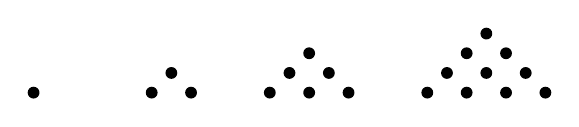
\begin{tikzpicture}[scale=0.5]
% T1 = 1
\foreach \x in {0} {
    \fill (\x,0) circle (0.15);
}
% Valor $T_1 = 1$ representado na figura

% T2 = 3
\begin{scope}[xshift=3cm]
\foreach \x in {0,1} {
    \fill (\x,0) circle (0.15);
}
\fill (0.5,0.5) circle (0.15);
% Valor $T_2 = 3$ representado na figura
\end{scope}

% T3 = 6
\begin{scope}[xshift=6cm]
\foreach \x in {0,1,2} {
    \fill (\x,0) circle (0.15);
}
\foreach \x in {0.5,1.5} {
    \fill (\x,0.5) circle (0.15);
}
\fill (1,1) circle (0.15);
% Valor $T_3 = 6$ representado na figura
\end{scope}

% T4 = 10
\begin{scope}[xshift=10cm]
\foreach \x in {0,1,2,3} {
    \fill (\x,0) circle (0.15);
}
\foreach \x in {0.5,1.5,2.5} {
    \fill (\x,0.5) circle (0.15);
}
\foreach \x in {1,2} {
    \fill (\x,1) circle (0.15);
}
\fill (1.5,1.5) circle (0.15);
% Valor $T_4 = 10$ representado na figura
\end{scope}
\end{tikzpicture}
\end{center}

\vspace{0.5cm}

\subexercicio{Represente os quatro primeiros termos da sucessao ($T_1, T_2, T_3, T_4$) em sistema binario.}

\subexercicio{Escreva o 5º termo da sucessao ($T_5$) em notacao decimal e hexadecimal.}

\subexercicio{Determine o 10º termo da sucessao ($T_{10}$) e represente-o em sistema binario.}

\subexercicio{Escreva a regra geral para gerar o proximo termo da sucessao dos numeros triangulares.}}

\FloatBarrier

% Exercise ID: MAT_A8MODELO_1SX_NFX_010
% Module: Módulo A8 - Modelos Discretos | Concept: Sistemas Numéricos | Type: Números Figurados
% Difficulty: 2/5 (Fácil) | Format: standard
% Tags: sistemas_numericos, hexadecimal, sequencias, binario, decimal
% Author: Test Agent | Date: 2025-11-27
% Status: active

\exercicio{Teste simples de números figurados - workflow completo}

\FloatBarrier

% Exercise ID: MAT_A8MODELO_1SX_NFX_011
% Module: Módulo A8 - Modelos Discretos | Concept: Sistemas Numéricos | Type: Números Figurados
% Difficulty: 2/5 (Fácil) | Format: standard
% Tags: hexadecimal, sistemas_numericos, decimal, binario, sequencias
% Author: Test Agent | Date: 2025-11-27
% Status: active

\exercicio{Teste simples de números figurados - workflow completo}

\FloatBarrier

% Exercise ID: MAT_A8MODELO_1SX_NFX_012
% Module: Módulo A8 - Modelos Discretos | Concept: Sistemas Numéricos | Type: Números Figurados
% Difficulty: 2/5 (Fácil) | Format: standard
% Tags: decimal, sequencias, binario, sistemas_numericos, hexadecimal
% Author: Test Agent | Date: 2025-12-02
% Status: active

\exercicio{Teste simples de números figurados - workflow completo}

\FloatBarrier

% Exercise ID: MAT_A8MODELO_1SX_NFX_012
% Module: Módulo A8 - Modelos Discretos | Concept: Sistemas Numéricos | Type: Números Figurados
% Difficulty: 3/5 (Médio) | Format: standard
% Tags: sistemas_numericos, binario, decimal, sequencias, hexadecimal, numeros_quadrados, representacao_visual, conversao_bases, regra_sucessao
% Author: Professor Diogo | Date: 2025-11-26
% Status: active

\exercicio{Observe a sucessão dos números quadrados representados visualmente abaixo (os valores $Q_1$, $Q_2$, $Q_3$, $Q_4$ estão indicados nas figuras):

\begin{center}
\begin{tikzpicture}[scale=0.4]
% Q1 = 1
\foreach \x in {0} {
    \foreach \y in {0} {
        \fill (\x,\y) circle (0.12);
    }
}
% Valor $Q_1 = 1$ representado na figura

% Q2 = 4
\begin{scope}[xshift=3cm]
\foreach \x in {0,1} {
    \foreach \y in {0,1} {
        \fill (\x,\y) circle (0.12);
    }
}
% Valor $Q_2 = 4$ representado na figura
\end{scope}

% Q3 = 9
\begin{scope}[xshift=7cm]
\foreach \x in {0,1,2} {
    \foreach \y in {0,1,2} {
        \fill (\x,\y) circle (0.12);
    }
}
% Valor $Q_3 = 9$ representado na figura
\end{scope}

% Q4 = 16
\begin{scope}[xshift=12cm]
\foreach \x in {0,1,2,3} {
    \foreach \y in {0,1,2,3} {
        \fill (\x,\y) circle (0.12);
    }
}
% Valor $Q_4 = 16$ representado na figura
\end{scope}
\end{tikzpicture}
\end{center}

\vspace{0.5cm}

\subexercicio{Represente os quatro primeiros termos da sucessao ($Q_1, Q_2, Q_3, Q_4$) em sistema hexadecimal.}

\subexercicio{Escreva o 5º termo da sucessao ($Q_5$) em notacao decimal e binaria.}

\subexercicio{Determine o 8º termo da sucessao ($Q_8$) e represente-o em sistema hexadecimal.}

\subexercicio{Escreva a regra geral para gerar o proximo termo da sucessao dos numeros quadrados.}}

\FloatBarrier

% Exercise ID: MAT_A8MODELO_1SX_NFX_013
% Module: Módulo A8 - Modelos Discretos | Concept: Sistemas Numéricos | Type: Números Figurados
% Difficulty: 4/5 (Difícil) | Format: standard
% Tags: binario, decimal, sequencias, hexadecimal, sistemas_numericos, numeros_pentagonais, representacao_visual, conversao_bases, regra_sucessao
% Author: Professor Diogo | Date: 2025-11-26
% Status: active

\exercicio{Analise a sucessão dos números pentagonais representados visualmente abaixo (os valores $P_1$, $P_2$, $P_3$, $P_4$ estão indicados nas figuras):

\begin{center}
\begin{tikzpicture}[scale=0.35]
% P1 = 1
\fill (0,0) circle (0.1);
% Valor $P_1 = 1$ representado na figura

% P2 = 5
\begin{scope}[xshift=3cm]
\foreach \i in {0,72,144,216,288} {
    \fill ({cos(\i)},{sin(\i)}) circle (0.1);
}
% Valor $P_2 = 5$ representado na figura
\end{scope}

% P3 = 12
\begin{scope}[xshift=7cm]
% Camada interior
\foreach \i in {0,72,144,216,288} {
    \fill ({cos(\i)},{sin(\i)}) circle (0.1);
}
% Camada exterior
\foreach \i in {0,72,144,216,288} {
    \fill ({2*cos(\i)},{2*sin(\i)}) circle (0.1);
}
% Valor $P_3 = 12$ representado na figura
\end{scope}

% P4 = 22
\begin{scope}[xshift=13cm]
% Camada interior
\foreach \i in {0,72,144,216,288} {
    \fill ({cos(\i)},{sin(\i)}) circle (0.1);
}
% Camada media
\foreach \i in {0,72,144,216,288} {
    \fill ({2*cos(\i)},{2*sin(\i)}) circle (0.1);
}
% Camada exterior
\foreach \i in {0,72,144,216,288} {
    \fill ({3*cos(\i)},{3*sin(\i)}) circle (0.1);
}
% Valor $P_4 = 22$ representado na figura
\end{scope}
\end{tikzpicture}
\end{center}

\vspace{0.5cm}

\subexercicio{Represente os quatro primeiros termos da sucessao ($P_1, P_2, P_3, P_4$) em sistema binario.}

\subexercicio{Escreva o 5º termo da sucessao ($P_5$) em notacao decimal e hexadecimal.}

\subexercicio{Determine o 7º termo da sucessao ($P_7$) e represente-o em sistema binario.}

\subexercicio{Escreva a regra geral para gerar o proximo termo da sucessao dos numeros pentagonais.}}

\FloatBarrier


\newpage


\end{document}
